\documentclass[handout]{beamer}
%\documentclass{beamer}
\usepackage[utf8]{inputenc}
\usepackage[T1]{fontenc}
\usepackage[francais]{babel}
\usepackage{eurosym}

\usetheme[opacity=0.0]{diepen}

\title{Développement du module d'annotation dans OOo Impress}
\author{Clément~\textsc{Delafargue} \and Morgan~\textsc{Magnin} \and Guillaume~\textsc{Moreau} \and Nelle~\textsc{Varoquaux}\and Benjamin~\textsc{Vialle}}
\institute[\textsc{ECN}]{École Centrale de Nantes}
\date{11 juillet 2011}



%\useinnertheme[shadow=false]{rounded}
\setbeamerfont{block title}{size={},series=\bfseries}


\setbeamercolor*{frametitle}{fg=black}
\setbeamercolor*{title}{fg=black}
\setbeamercolor*{subtitle}{fg=black}
\setbeamercolor*{author}{fg=black}
\setbeamercolor*{institute}{fg=black}
\setbeamercolor*{date}{fg=black}
\usecolortheme[named=black]{structure}
\setbeamercolor{alerted text}{fg=black}
\setbeamercolor{block title}{fg=black}
\setbeamercolor{block title example}{fg=black!90!black}
\setbeamercolor{normal text}{fg=black}
%\useoutertheme{shadow}

\begin{document}

\frame{\titlepage}

\section{Contexte}

\begin{frame}{Centrale Nantes et le Libre}
    \begin{block}{Collaborations}
	\begin{itemize}[<+->]
	    \item MarkUs
	    \item OrbisGis (\textit{via} IRSTV)
	    \item OpenOffice.org OpenOffice.org4Kids
	\end{itemize}
    \end{block}
\end{frame}

\begin{frame}{OOo/OOo4Kids à Centrale Nantes}
    \begin{block}{Concours HP - 21 Tablet PCs gagnés en 2008}
	\begin{itemize}[<+->]
	    \item Cartable électronique libre
            \item GNU/Linux
            \item Amélioration d'OpenOffice.org Impress pour les Tablet-PCs
	\end{itemize}
    \end{block}
\end{frame}

\begin{frame}{OOo/OOo4Kids à Centrale Nantes}
    \begin{block}{Module d'annotation dans OpenOffice}
	\begin{itemize}
	    \item Codé en C++
	    \item Possibilité de changer
	    \begin{itemize}
		\item taille
		\item couleur
	    \end{itemize}
	\end{itemize}
    \end{block}
\end{frame}

\begin{frame}{OOo/OOo4Kids à Centrale Nantes}
    \begin{block}{OOo4Kids}
	\begin{itemize}[<+->]
	    \item Logiciel de bureautique libre et gratuit pour les 7-12 ans
	    \item OpenOffice.org simplifié
	    \item Adapté aux programmes d'enseignement.
	\end{itemize}
    \end{block}
\end{frame}

\begin{frame}{Module d'annotations}
    \begin{block}{2009}
        \begin{itemize}[<+->]
            \item Gomme
	    \item Sauvegarde des annotations
        \end{itemize}
    \end{block}
\end{frame}

\begin{frame}{Module d'annotations}
    \begin{block}{2010}
        \begin{itemize}[<+->]
            \item Debogage des patchs des années précédentes
	    \item Switch entre gomme et crayon
        \end{itemize}
    \end{block}
\end{frame}

\begin{frame}{Module d'annotations}
    \begin{block}{2011: Objectifs}
        \begin{itemize}[<+->]
            \item Mode curseur
            \item Extensibilité
        \end{itemize}
    \end{block}
\end{frame}

\section{Cadre Technique}

\begin{frame}{Travail préliminaire}
    \begin{block}{Documentation}
        \begin{itemize}[<+->]
            \item Rapports des années précédentes
            \item Wiki OOo4Kids
            \item Conventions de codage
            \item Documentation Libre Office
        \end{itemize}
    \end{block}
\end{frame}

\begin{frame}{Travail préliminaire}
    \begin{block}{Cahier des charges}
        \begin{itemize}[<+->]
            \item Maquettes UI
            \item Diagrammes d'état
        \end{itemize}
    \end{block}
\end{frame}

\begin{frame}{Travail préliminaire}
    \begin{block}{Environnement de développement}
        \begin{itemize}[<+->]
            \item Compilation (dmake, ccache, distcc)
            \item Debian, Ubuntu, Gentoo
            \item Versionnement (SVN, Hg, Git)
        \end{itemize}
    \end{block}
\end{frame}

\begin{frame}{Démarche de développement}
    \begin{block}{Mimétisme}
        \begin{itemize}[<+->]
            \item Modifications minimales
            \item Reprise des structures existantes 
            \item Respect de la localité
        \end{itemize}
    \end{block}
\end{frame}

\begin{frame}{Démarche de développement}
    \begin{block}{Pattern commando}
        \begin{itemize}[<+->]
            \item grep sauvage
            \item Modifications minimales et localisées
        \end{itemize}
    \end{block}
\end{frame}

\begin{frame}{Démarche de développement}
    \begin{block}{3 phases}
        \begin{itemize}[<+->]
            \item Logique métier
            \item Interface utilisateur
            \item Branchements
        \end{itemize}
    \end{block}
\end{frame}

\begin{frame}{Assurance Qualité}
    \begin{block}{Documentation}
        \begin{itemize}[<+->]
            \item Comptes-rendus réguliers
            \item Peu de choix à expliciter
        \end{itemize}
    \end{block}
\end{frame}

\begin{frame}{Assurance Qualité}
    \begin{block}{Revue de code}
        \begin{itemize}[<+->]
            \item Patches courts
            \item Revue effectuée par Éric
            \item Pair programming = revue "à la volée"
        \end{itemize}
    \end{block}
\end{frame}

\begin{frame}{Assurance Qualité}
    \begin{block}{Critères à respecter}
        \begin{itemize}[<+->]
            \item Compilation sans warnings
            \item Patches cohérents
        \end{itemize}
    \end{block}
\end{frame}

\section{Cadre pédagogique}

\begin{frame}{Cadre pédagogique}
    \begin{block}{Encadrants}
        \begin{itemize}[<+->]
            \item Tuteur enseignant~: Morgan Magnin
            \item Mentor technique~: Éric Bachard
        \end{itemize}
    \end{block}
\end{frame}

\begin{frame}{Cadre pédagogique}
    \begin{block}{Anciens élèves}
        \begin{itemize}[<+->]
            \item Rapports
            \item Retours d'expérience
        \end{itemize}
    \end{block}
\end{frame}

\begin{frame}{Cadre pédagogique}
    \begin{block}{Communication}
        \begin{itemize}[<+->]
            \item Wiki
            \item IRC
            \item Blog
        \end{itemize}
    \end{block}
\end{frame}

\section{Bilan}
\begin{frame}{Difficultés}
    \begin{block}{Processus lourd}
        \begin{itemize}[<+->]
            \item Compilation difficile
            \item Temps de compilation importants
            \item Intégration compliquée
        \end{itemize}
    \end{block}
\end{frame}

\begin{frame}{Difficultés}
    \begin{block}{Base de code de qualité inégale}
        \begin{itemize}[<+->]
            \item Cohérence faible
            \item Code mal commenté
        \end{itemize}
    \end{block}
\end{frame}

\begin{frame}{Difficultés}
    \begin{center}
    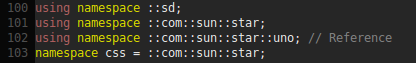
\includegraphics[scale=0.5]{images/screenshot_032.png}
    \end{center}    
\end{frame}

\begin{frame}{Difficultés}
    \begin{center}
    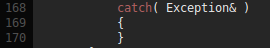
\includegraphics[scale=0.5]{images/screenshot_033.png}
    \end{center}    
\end{frame}

\begin{frame}{Difficultés}
    \begin{center}
    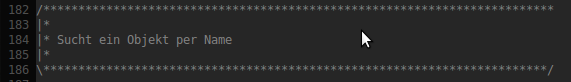
\includegraphics[scale=0.5]{images/screenshot_034.png}
    \end{center}    
\end{frame}

\begin{frame}{Difficultés}
    \begin{center}
    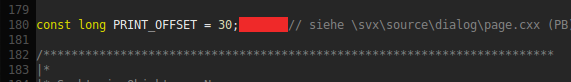
\includegraphics[scale=0.5]{images/screenshot_035.png}
    \end{center}    
\end{frame}

\begin{frame}{Difficultés}
    \begin{center}
    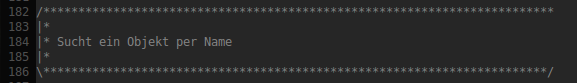
\includegraphics[scale=0.5]{images/screenshot_036.png}
    \end{center}    
\end{frame}

\begin{frame}{Difficultés}
    \begin{center}
    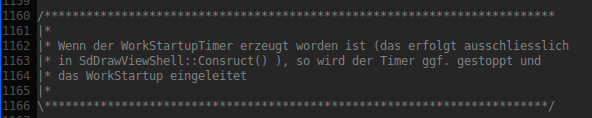
\includegraphics[scale=0.5]{images/screenshot_037.png}
    \end{center}    
\end{frame}

\begin{frame}{Difficultés}
    \begin{center}
    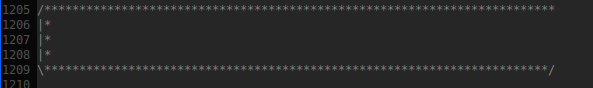
\includegraphics[scale=0.5]{images/screenshot_038.png}
    \end{center}    
\end{frame}

\begin{frame}{Difficultés}
    \begin{center}
    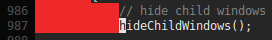
\includegraphics[scale=0.5]{images/screenshot_039.png}
    \end{center}    
\end{frame}

\begin{frame}{Apports}
    \begin{block}{Projet libre}
        \begin{itemize}[<+->]
            \item Code publié
            \begin{itemize}[<+->]
                \item Valorisation
                \item Assurance qualité
            \end{itemize}
            \item Satisfaction personnelle
            \item "Gros" projets
        \end{itemize}
    \end{block}
\end{frame}

\begin{frame}{Apports}
    \begin{block}{Gros projet}
        \begin{itemize}[<+->]
            \item Connu, reconnu
            \item Base de code importante
            \item Processus stricts
        \end{itemize}
    \end{block}
\end{frame}

\begin{frame}{Bilan}
    \begin{block}{Caractéristiques communes}
        \begin{itemize}[<+->]
            \item Petits patches
            \item Travail important
        \end{itemize}
    \end{block}
\end{frame}

\begin{frame}{Bilan}
    \begin{block}{Perspectives}
        \begin{itemize}
            \item Intégration à OpenOffice.org et/ou LibreOffice
            \item Améliorations
            \item Documentation
        \end{itemize}
    \end{block}
\end{frame}

\begin{frame}{Bilan}
    \begin{block}{}
        \begin{center}
            Questions ?
        \end{center}
    \end{block}
\end{frame}


\end{document}
